\documentclass[border=10pt]{standalone}
\usepackage{pgfplots}
\pgfplotsset{width=7cm,compat=1.8}
\usepgfplotslibrary{polar}
\begin{document}
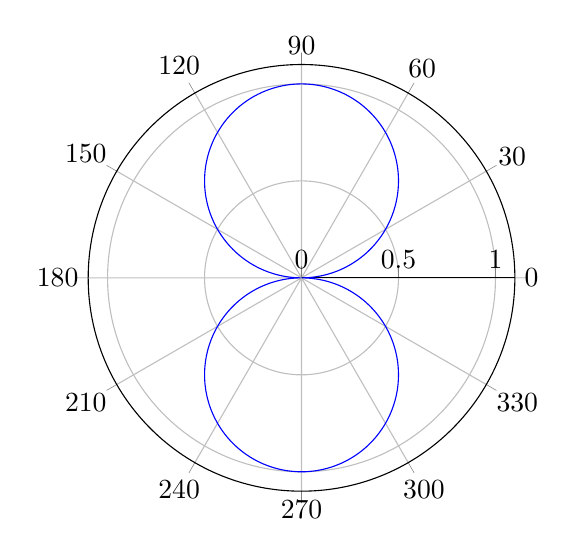
\begin{tikzpicture}
	\begin{polaraxis}
	\addplot+[mark=none,domain=0:720,samples=600] 
		{abs(sin(x))}; 
	% equivalent to (x,{sin(..)cos(..)}), i.e.
	% the expression is the RADIUS
	\end{polaraxis}
\end{tikzpicture}
\end{document}